% \part{Template}\label{part:appendices}
\chapter{A Cavity-based Network Design}\label{ch:cavitynode}

In light of the analysis in \cite{Young2022}, we had planned to implement a cavity version of the network experiment. One of the main bottlenecks in the remote entanglement generation rate for a quantum network is the photon collection efficiency, which can approach unity by placing the communication qubits in a suitable optical cavity. By using a cavity operated in the near-concentric regime, i.e. with length $L$ just below twice the mirror radii of curvature $R$, a small mode waist can be obtained while maintaining a relatively large mirror separation. This means that we acheive a strong interaction between the an atom and the cavity mode while avoiding deleterious effects associated with short cavities such as the accumulation surface charges which can induce significant Stark shifts on Rydberg states \cite{Bohorquez2023}. Moroever, the cavity length allows for increased optical access, allowing, e.g., for forming a MOT within the cavity. This appendix presents the mechanical and optical design for cavity-based network node, for which all of the main parts have been ordered. The project is on-pause as of the time of this writing, as the lab pivots toward dual-species remote entanglement.

\section{Cavity Mirrors}\label{sec:cavmirrors}

The cavities were designed to simultaneously support modes at 780 nm and 1540 nm, the wavelengths of the emitted photons for networking and cavity lock reference, respectively. Depending on the choice of phases imparted by the mirror coatings, the nodes and anti-nodes of standing waves at these two wavelengths can line up in different ways, as is described in \cite{garcia2020overlapping}. By suitable choice of these phases, the 1540 field can be used to provide tight axial confinement of atoms within the pancakes shaped high intensity regions formed by antinodes in the standing wave. The analysis to calculate the mirror coating phases was done by Akbar Safari.

\begin{figure}[!ht]
    \centering
    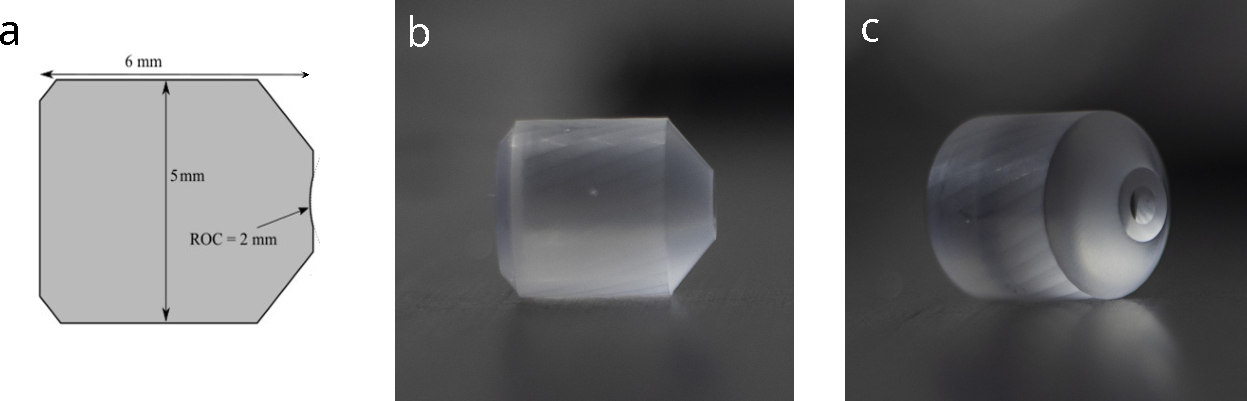
\includegraphics[width=0.9\textwidth]{Images/cavity_mirror_substrate.pdf}
    \caption{The fused silica cavity mirror substrate design and photos of the final product from Optics Technology in Rochester, NY. The chamfered edges allow clearance for $\sim1$ mm diameter MOT beams to be sent through the cavity. Design image and photos courtesy of Akbar Safari.}
    \label{fig:cavmirror_substrate}
\end{figure}

The cavity is designed to be ``one-sided" at 780 nm, such that nearly all of the photons emitted from the atom exit through only one of the two mirrors. The 1540 nm laser used for the cavity lock will be coupled into the cavity through the other mirror. 

\section{Mode Matching}\label{sec:cavmatching}

Mode matching light to a near-concentric cavity involves converting an incident plane wave (i.e. a collimated beam) into a spherical wave which focuses down to the cavity waist, which is accomplished optimally by using a cavity mirror whose back surface is elliptical \cite{Durak_2014}. However, for ease of budget and design complexity, we can approximate such a monolithic mirror substrate with by a flat-back cavity mirror and a plano-convex lens, placed nearly back to back (Fig. (\ref{fig:modematchapprox})). 

\begin{figure}[!ht]
    \centering
    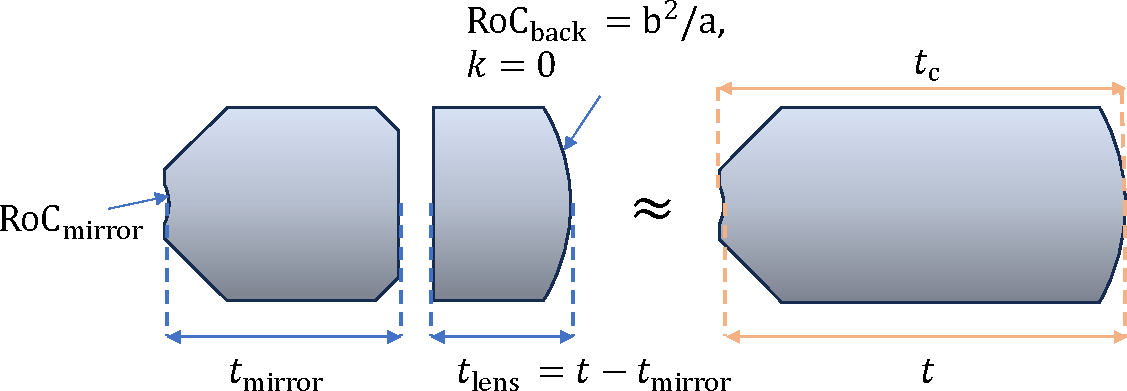
\includegraphics[width=0.9\textwidth]{Images/mode_matching_mirror_approximation.pdf}
    \caption{A cavity mirror with an elliptical back surface (right) for transforming a spherical wave in the cavity to a plane wave outside the cavity can be approximated by a mirror with a flat back plus a plano-convex spherical lens (left). The spherical surface of the lens should have the same curvature constant as the elliptical surface. See text for details.}
    \label{fig:modematchapprox}
\end{figure}

The curvature of optical surface, or sag, for a conic surface $i$ ($i=1$ is the mirror surface, $i=2$ is the back surface) is given by 
\begin{equation}\label{eq:sag}
    sag_i(r) = \frac{c_i r^2}{1+\sqrt{1 - (1+k) c_i^2 r^2}} 
\end{equation}
where $c$, $k$, and $r$ are the curvature, conic constant, and radius from the optical axis. For the desired elliptical surface, we have $c=a/b^2$ and $k=(b^2-a^2)/a^2$ in which $b=f \sqrt{(n-1)/(n+1)}$, $a = f n/(n+1)$, where $n$ is the index of refraction of the mirror substrate and $f$ its effective focal length. Taylor expanding Eq. (\ref{eq:sag}) gives
\begin{equation}
    \frac{c r^2}{2} + \frac{c^3 r^4}{8} + \frac{k c^3 r^4}{8} + \mathcal{O}(r^5).
\end{equation}
For $f=10 mm$, $n=1.765$ (Fused Silica at 780 nm), and $r=0.5 mm$ (clear aperture), a spherical surface ($k=0$) deviates from a spherical one on the order of $10^{-4}$, justifying our approximation.

We want to solve for parameters for two lenses, one to approximate the role of an elliptical surface for mode-matching to the cavity, and one for coupling to match the collimated cavity output to a fiber.

For a given desired cavity mode waist $w_0$ at wavelength $\lambda$; and mirror substrate $n$ and thickness $t$ (if monolothic mirror $+$ elliptical surface) and clear aperture $r_{CA}$,  we can compute the effective focal length $f$. Note that $t$ is chosen to be the thickness of the flat-back mirror substrate plus some additional thickness to account for that of the lens we will use to approximate the elliptical surface. We then solve the following two equations:
\begin{align} 
    t_c &= t - sag_1(r_{CA}) \\ 
    f &= t_c + 1/c_1  
\end{align}
with $c_1$ equal to the reciprocal of the mirror radius of curvature and $t_c$ is the total center thickness.

The effective focal length of a lens with thickness $d$ is given by
\begin{equation}
    efl = \frac{1}{(n-1)(c_1 - c_2 + \frac{c_1 c_2 (n-1)d}{n})}
\end{equation}
where $c_1=0$ for a plano-convex lens. To approximate an elliptical surface, we want the spherical side have to R.o.C. of $ -1/c_2 = b^2/a$, which depends on $f$ which can be solved for as shown above.

The required fiber coupling lens focal length is found by using the waist transformation for Gaussian beams, starting with the cavity waist. The waist on the back surface of the monolithic mirror is
\begin{equation}
    w_1 = \frac{\lambda f}{w_0 \pi}
\end{equation}
and the required fiber coupling lens focal length is
\begin{equation}
    f_c = \frac{\pi w_1 w_{\textrm{fiber}}}{\lambda}.
\end{equation}

Mathematica code for this procedure of calculating mode matching lenses is available upon request. This procedure was used for picking candidate off-the-shelf lenses, which were then checked in Zemax with a model of the flat-backed mirror substrate for fiber coupling and mode matching efficiency at the design wavelengths. 

Lenses were chosen for a cavity waist of $8~\mu $m 780 nm, correpsonding to a cavity length which deviates from near-concentric by $67.5~\mu m$ (i.e. the critical distance) and with fused silica mirror substrates with 6 mm thickness, and mirror RoC 2 mm and clear aperture 0.5 mm (Fig. \ref{fig:cavmirror_substrate}). Simulations in Zemax using Physical Optics Propagation were done to compute the fiber coupling efficiency for the 780 nm mode emitted by the cavity and mode-matching efficiency for 1560 nm light launched from a SM fiber, where the results are tabulated in Fig. \ref{fig:modematchdesign}. The spacings between lenses were optimized for the best efficiencies. For the same set of lenses and spacings, the calculations were repeated for two different 780 nm waist values (corresponding to different cavity lengths in the simulation) to see how forgiving the design is at cavity lengths which are increasingly more stable.

\begin{figure}[!ht]
    \centering
    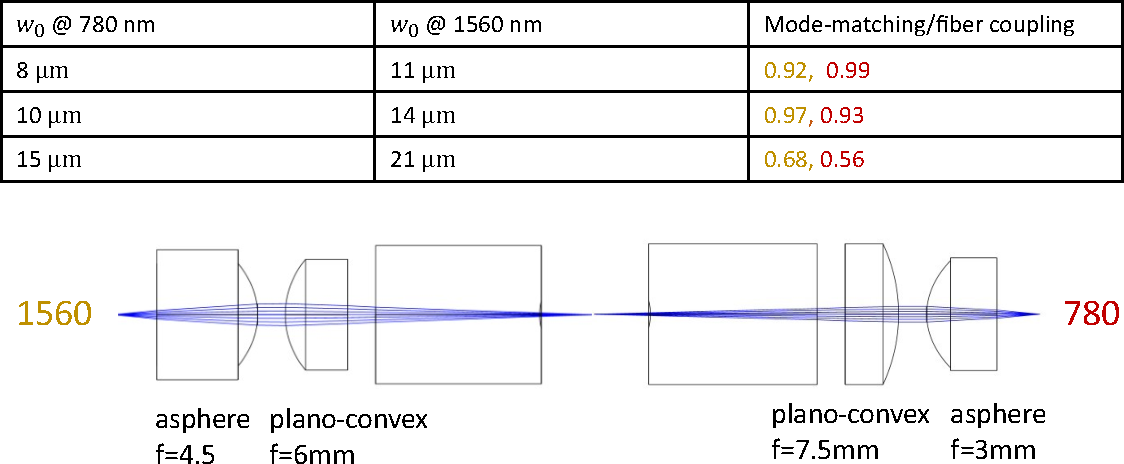
\includegraphics[width=0.9\textwidth]{Images/zemax_cavity_design.pdf}
    \caption{Mode matching lenses for coupling a 1560 nm beam from a SM fiber into the cavity, and a cavity mode at 780 nm out of the cavity and into an SM fiber. The lenses are, from left to right, \href{https://www.edmundoptics.com/p/043-na-450mm-fl-1050-1600nm-ar-coated-molded-aspheric-lens/26661/}{Edmund 83-580}, \href{https://www.edmundoptics.com/p/40mm-dia-x-60mm-fl-nir-ii-coated-plano-convex-lens/21908/}{Edmund 67-447}, \href{https://www.edmundoptics.com/p/50mm-diameter-x-75mm-fl-785nm-v-coat-pcx-lens/31486/}{Edmund 89-014}, and \href{https://www.thorlabs.com/thorproduct.cfm?partnumber=355660-B}{Thorlabs 355660-B}. Hyperlinks to products are available online.}
    \label{fig:modematchdesign}
\end{figure}

\section{Cavity opto-mechanics}\label{sec:cavopto}

The mechanical design of the cavity uses Macor housings to secure the cavity mirror substrates, mode-matching lenses, fiber coupling lenses, and ferrules for optical fibers. The fiber coupling lenses and fiber ferrule are held in a separate housing from the mode-matching lens and cavity mirror to allow for relative alignment tuning or the option to forego a fiber-coupled cavity in favor of free space mode-matching on either or both sides of the cavity. This design is shown for both cavity sides in Fig. \ref{fig:modematchhousings} for the optics in Fig. \ref{fig:modematchdesign}.

\begin{figure}[!ht]
    \centering
    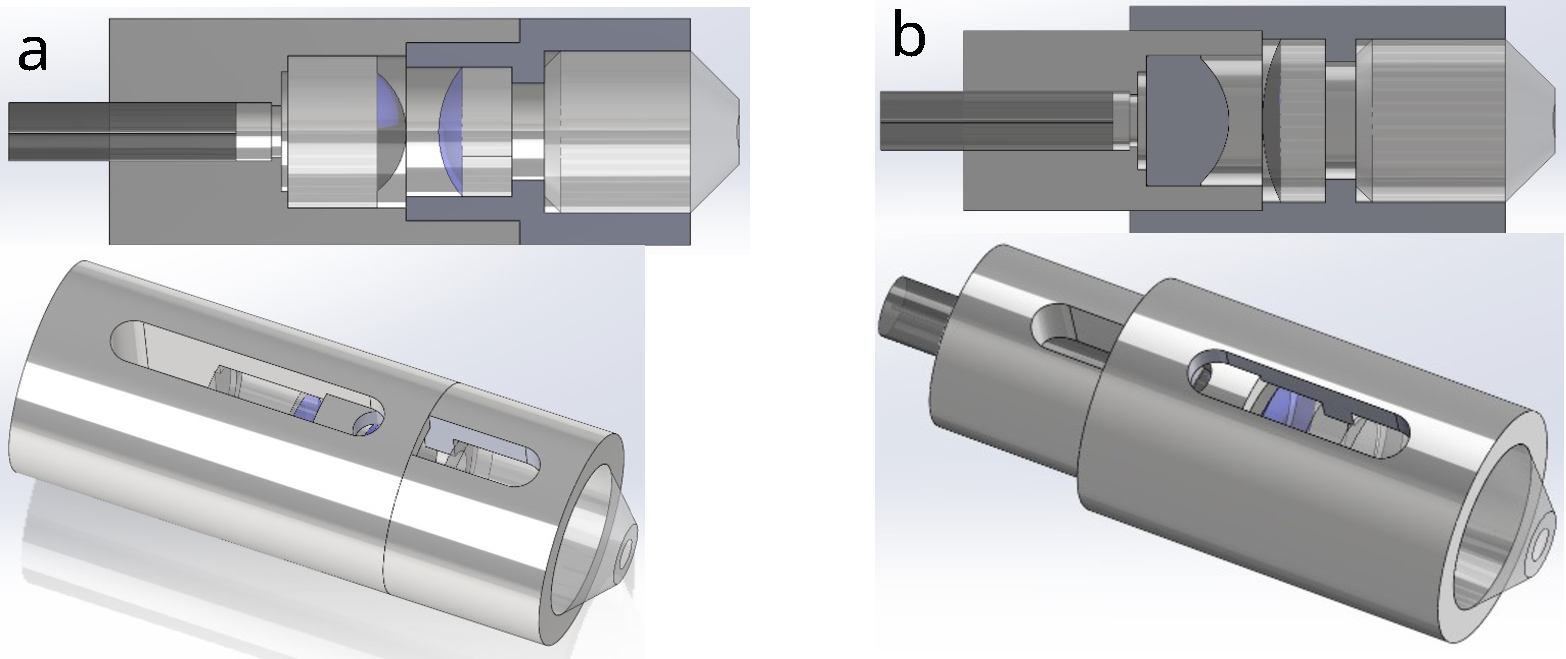
\includegraphics[width=0.9\textwidth]{Images/mode_matching_housings.pdf}
    \caption{Solidworks models of the housings designed to mount the fiber and cavity mode matching optics to the cavity mirrors for both the 780 nm photon collection side (\textbf{b}) and the 1560 nm locking side (\textbf{a}). The housings are designed to be Macor and are vented for use in vacuum. Note: the models shown were modified after the above images were made to include a chamfer on the cavity mirror end of each housing to match the cavity mirror's own chamfer, in order to not clip MOT beams. This update can be seen in Fig. \ref{fig:cavitybridge}.}
    \label{fig:modematchhousings}
\end{figure}

The entire cavity assembly can be mounted in Macor V-groove pieces which themselves are mounted on a linear alignment piece or "bridge" which holds the entire cavity together once the individual optic housing and V-grooves have been aligned and glued. The cavity mirror housing V-grooves are in turn mounted to shear-mode piezo-electric transducers (Noliac NAC2402-H3.4). The exact height of the cavity mirror may need to be adjusted, which can be done by shimming the V-grooves on one side of the cavity. For this purpose, titanium shims (Surepure Chemetals) were ordered, as titanium and Macor have very similar coefficents of thermal expansion, which maintain the this similarity and the same sign over the range of temperatures including our vacuum bakeout. This design is shown in Fig. \ref{fig:cavitybridge} with an alternative fiber coupling housing design allowing for the insertion of $45^{\circ}$ mirrors to be inserted if switching to free-space mode-matching is desired. This allows for a plan B if fiber coupling becomes misaligned, for example, while the glue cures.
\begin{figure}[!ht]
    \centering
    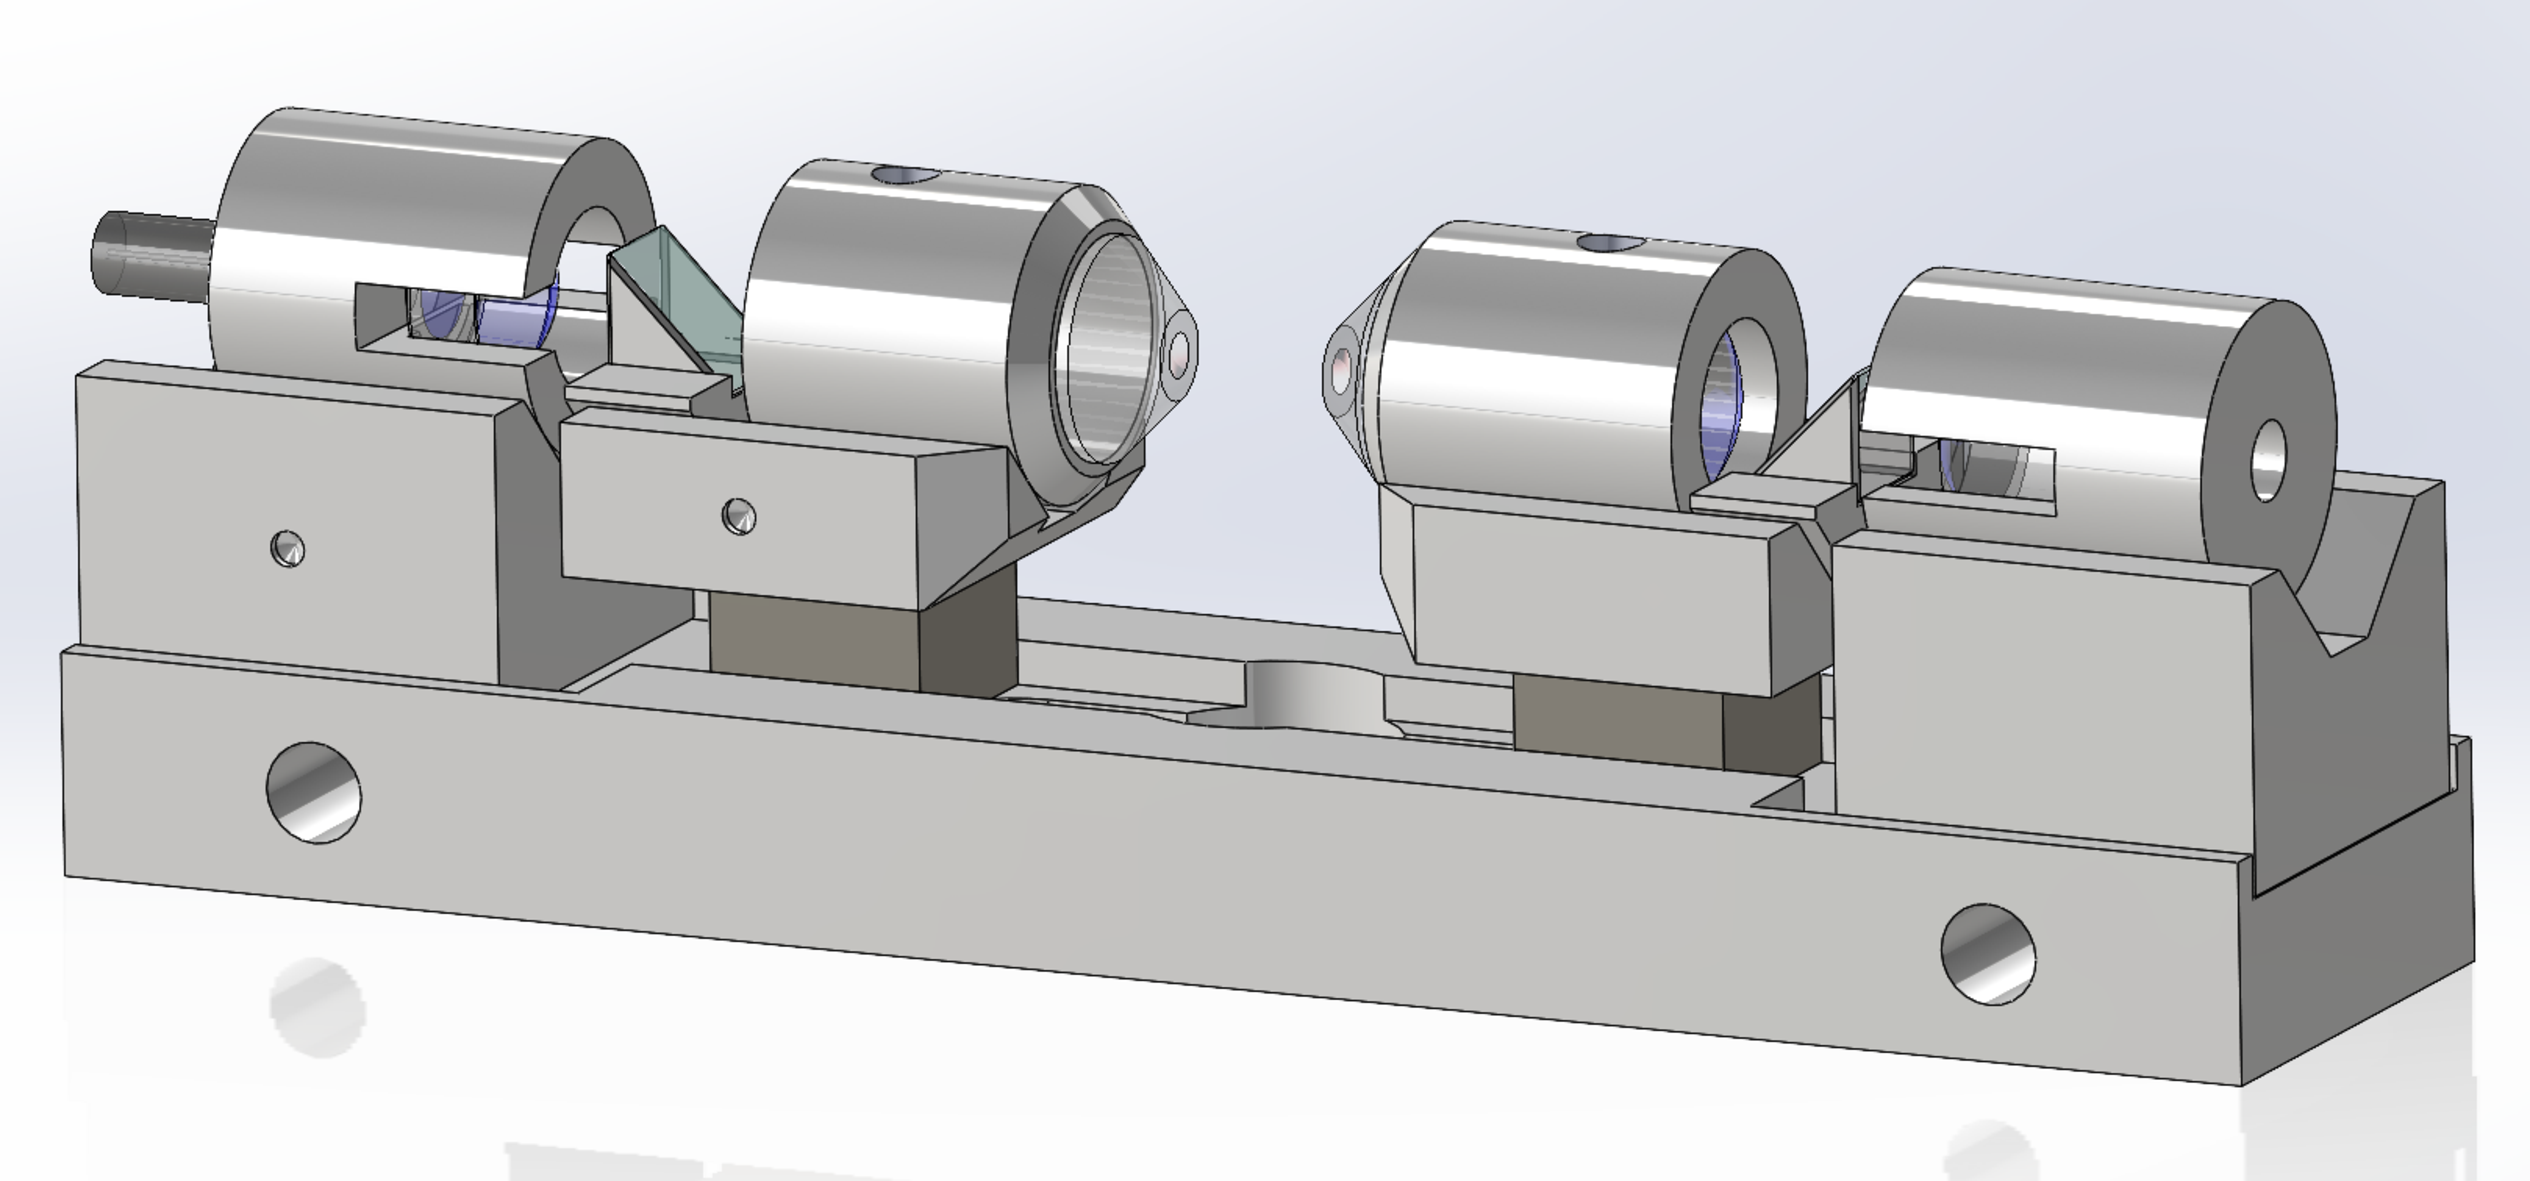
\includegraphics[width=0.45\textwidth]{Images/cavitybridge.pdf}
    \caption{Solidworks models of the assembled cavity with optional mirrors inserted between the fiber coupling and mode-matching optics housings on each side, to allow for free-space cavity coupling. The cavity length can be modulated using piezo-electric elements (dark gray). Note that the V-grooves on the left have small dimples to mark that they are 100 $\mu$m shorter vertically, to allow for shimming to the correct height.}
    \label{fig:cavitybridge}
\end{figure}

\section{MInt Chip}\label{sec:mintchip}

Some pics of the MInt chip and the chamber maybe ??


    


